%%%%%%%%%%%%%%%%%%%%%%%%%%%%%%%%%%%%%%%%%%%%%%%%%%%%%%%%%%%%%%%%%%%%%%%%%%%%%%%%
%2345678901234567890123456789012345678901234567890123456789012345678901234567890
%        1         2         3         4         5         6         7         8

\documentclass[letterpaper, 10 pt, conference]{ieeeconf}  % Comment this line out if you need a4paper

%\documentclass[a4paper, 10pt, conference]{ieeeconf}      % Use this line for a4 paper

\IEEEoverridecommandlockouts                              % This command is only needed if 
                                                          % you want to use the \thanks command

\overrideIEEEmargins                                      % Needed to meet printer requirements.

% See the \addtolength command later in the file to balance the column lengths
% on the last page of the document

% The following packages can be found on http:\\www.ctan.org
%\usepackage{graphics} % for pdf, bitmapped graphics files
%\usepackage{epsfig} % for postscript graphics files
%\usepackage{mathptmx} % assumes new font selection scheme installed
%\usepackage{times} % assumes new font selection scheme installed
%\usepackage{amsmath} % assumes amsmath package installed
%\usepackage{amssymb}  % assumes amsmath package installed
\title{\LARGE \bf
Learning Proposal Distributions for Refining High-Level Plans
}


\author{rohan$^{1}$, dylan$^{2}$, and pieter$^{2}$% <-this % stops a space
\thanks{$^{1}$\ \tt \small ronuchit@berkeley.edu}%
\thanks{$^{2}$\{\tt \small dhm, pabbeel\}@eecs.berkeley.edu}%
}

%% \usepackage[numbers]{natbib}
\usepackage{multicol}
\usepackage[bookmarks=true]{hyperref}
\usepackage{color}
\usepackage{amssymb}
\usepackage{amsmath}

%% \usepackage{amsthm}
\usepackage{booktabs}
\usepackage{graphicx}

\usepackage{caption}
\usepackage{subcaption}
%%\usepackage{subfigure}

\usepackage{algorithm2e}

\DeclareMathOperator*{\argmin}{argmin}
\DeclareMathOperator*{\argmax}{argmax}

\newenvironment{tightlist}%
{\begin{list}{$\bullet$}{%
    \setlength{\topsep}{0in}
    \setlength{\partopsep}{0in}
    \setlength{\itemsep}{0in}
    \setlength{\parsep}{0in}
    \setlength{\leftmargin}{1.5em}
    \setlength{\rightmargin}{0in}
    \setlength{\itemindent}{-.1in}
}
}%
{\end{list}
}

% \setlength{\parskip}{1pc}
% \setlength{\parindent}{0pt}
% \setlength{\topmargin}{-3pc}
% \setlength{\textheight}{9.5in}
% \setlength{\oddsidemargin}{0pc}
% \setlength{\evensidemargin}{0pc}
% \setlength{\textwidth}{6.5in}

\newcommand{\secref}[1]{Section~\ref{#1}}
\newcommand{\exref}[1]{Example~\ref{#1}}
\newcommand{\eqnref}[1]{Equation~\ref{#1}}
\newcommand{\figref}[1]{Figure~\ref{#1}}
\newcommand{\algoref}[1]{Algorithm~\ref{#1}}

\newcommand{\dhm}[1]{{\bf \textcolor{red}{Dylan: #1}}}

\newtheorem{thm}{Theorem}
\newtheorem{lem}{Lemma}
\newtheorem{defn}{Definition}
\newtheorem{conj}{Conjecture}
\newtheorem{cor}{Corollary}
\newtheorem{ex}{Example}

\newcommand{\ibsp}{\textsc{ibsp}}

\newcommand{\aml}{\textsc{aml}}
\newcommand{\mld}{\textsc{mld}}

\newcommand{\Obj}{\mathcal{O}}
\newcommand{\F}{\mathcal{F}}
\newcommand{\I}{\mathcal{I}}
\newcommand{\G}{\mathcal{G}}
\newcommand{\C}{\mathcal{C}}
\newcommand{\Prob}{\mathcal{P}}
\newcommand{\St}{\mathcal{S}}
\newcommand{\A}{\mathcal{A}}
\newcommand{\T}{\mathcal{T}}
\newcommand{\Gr}{\mathcal{G}}
\newcommand{\V}{\mathcal{V}}
\newcommand{\E}{\mathcal{E}}

\begin{document}

\bibliographystyle{IEEEtran}

\maketitle
\thispagestyle{empty}
\pagestyle{empty}


%%%%%%%%%%%%%%%%%%%%%%%%%%%%%%%%%%%%%%%%%%%%%%%%%%%%%%%%%%%%%%%%%%%%%%%%%%%%%%%%
\begin{abstract}
A key challenge in robotics is the execution of long-horizon tasks. These
require the robot to reason through a long sequence of high level steps in order to reach
a goal, as well as determine appropriate joint trajectories for executing each step.
Recent work has been devoted to hierarchical planning, which seeks
to plan for such goals by combining task and motion planning. These planning systems
attempt to refine symbolic plans by
searching for a feasible assignment of continuous values to the symbolic parameters. A core limitation
of task and motion planning systems is the manner in which values are sampled for the search:
using hand-coded distributions that leverage specificity about the geometry of the environment
and its objects. In this paper, we apply
techniques in reinforcement learning to train a system that produces good proposal
distributions for sampling plan parameter values. Our contributions are: 1) a machine learning
approach to find sampling distributions for the refinement of symbolic plans in
a hierarchical planning system; and 2) a
novel strategy for refining these symbolic plans based on randomization, which we found integrates well
with our learning algorithm. Our experiments demonstrate comparable to improved performance in motion planning
time and number of motion planner calls in a variety of test environments, when compared
to an existing baseline system that uses hand-tuned discrete sampling distributions.
\end{abstract}



%%%%%%%%%%%%%%%%%%%%%%%%%%%%%%%%%%%%%%%%%%%%%%%%%%%%%%%%%%%%%%%%%%%%%%%%%%%%%%%%
\section{Introduction}
We are interested in designing autonomous systems to perform complex
mobile manipulation tasks over long time horizons (e.g., setting a
dinner table, doing laundry). We approach this problem in the
framework of combined \emph{task and motion planning} ({\sc tamp}).

In {\sc tamp}, an agent is given a symbolic, logical characterization
of actions (e.g., move, grasp, putdown), along with a geometric
encoding of the environment.  Efficient integration of high-level,
symbolic task planning and low-level, geometric motion planning in {\sc tamp} is
difficult; recent research has proposed several
approaches~\cite{srivastava2014combined, deardenplanningtamp,
  kaelbling2011hierarchical, lagriffoul2014orientation,
  dornhege2012semantic, GarrettWAFR14}.  In this paper, we adopt the abstraction
framework developed by Srivastava et al.~\cite{srivastava2014combined}
(henceforth referred to as {\sc sfrcra-14}) to factor the reasoning
and search problems into interacting logical and geometric components.

\begin{figure}[t]
  \centering
    \noindent
    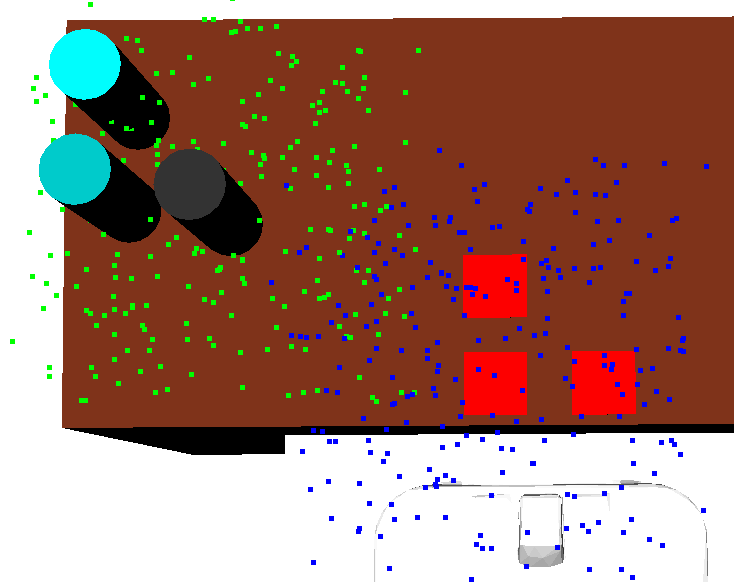
\includegraphics[scale=0.112]{images/learns.png}
    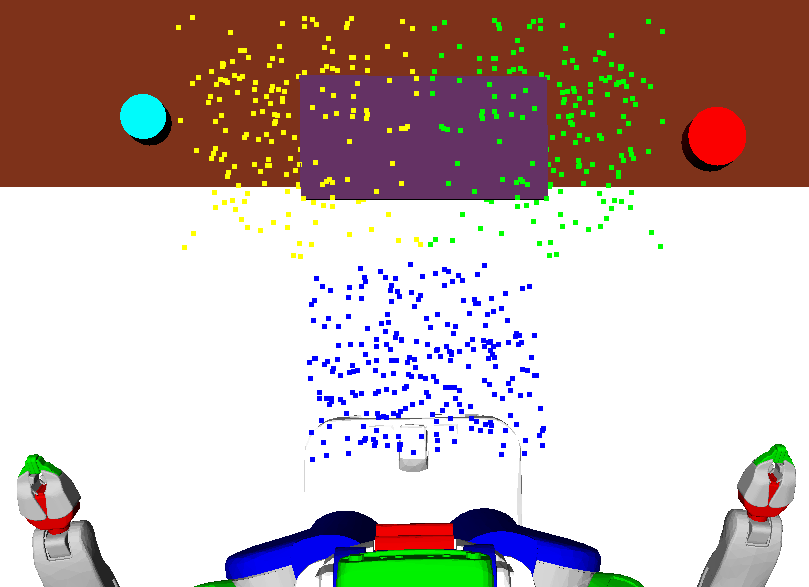
\includegraphics[scale=0.13]{images/dinner_tray_initial.png}
    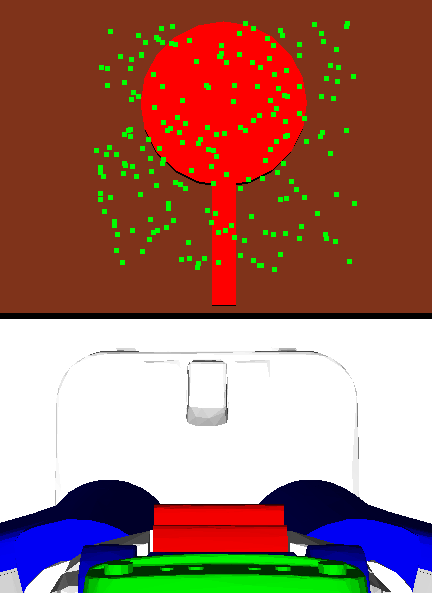
\includegraphics[scale=0.13]{images/frying_initial.png}\vspace{1em}
    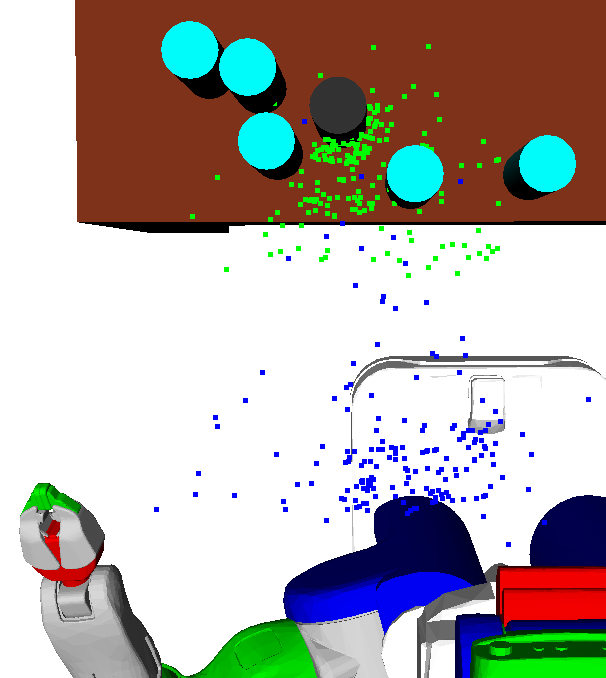
\includegraphics[scale=0.112]{images/learn12.png}
    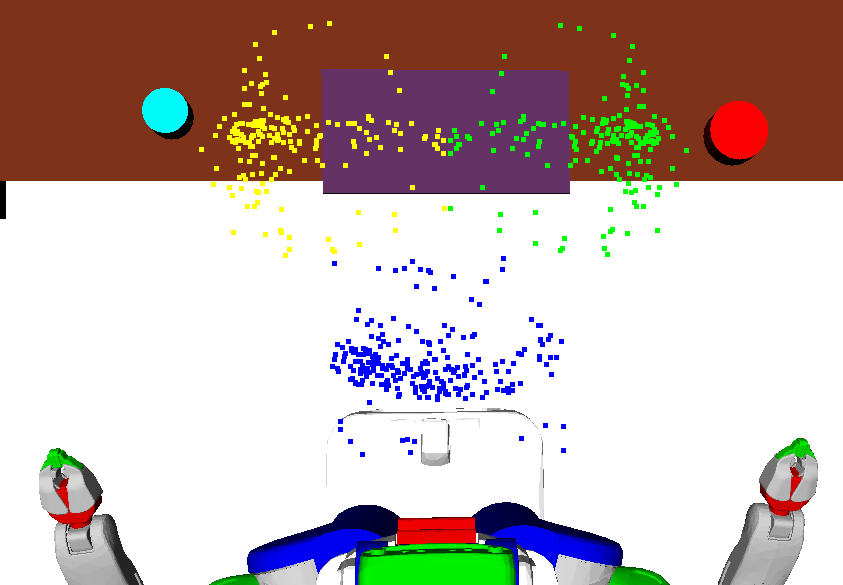
\includegraphics[scale=0.13]{images/dinner_tray_final.png}
    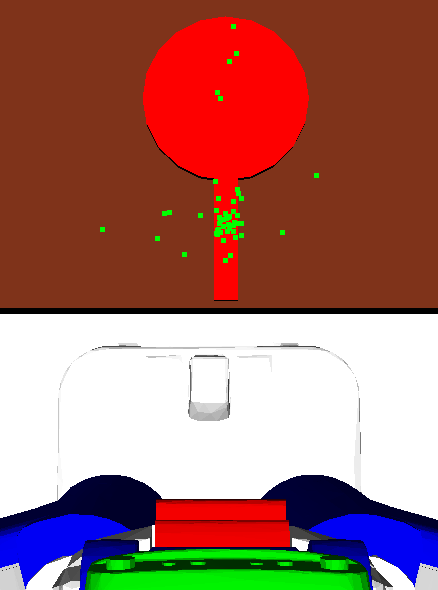
\includegraphics[scale=0.13]{images/frying_final.png}
  \caption{\small{We apply reinforcement learning to speed up planning
      for {\sc tamp} tasks. We break the problem down into a low-level
      policy that samples promising values for continuous parameters
      (e.g., pre-grasp poses, grasping poses, etc.), and a high-level
      policy that ranks different high-level plans. The above figures
      illustrate learning for the low-level system. The top images
      show initial, uniform distributions. The bottom images show
      learned distributions over base pose (blue) and end effector
      pose (green, yellow) for pick tasks in our simulated domains: a
      can (left), a tray (middle), and a frying pan (right).  The
      green and yellow points refer to the positions of the tool
      center points; the end effectors are oriented to point toward
      the object being grasped. The can and frying pan are picked up
      using only one gripper.}}
  \label{fig:cover}
\end{figure}

In this work, we develop a complete algorithm for {\sc tamp} and
propose learning methods to guide a joint search in the space of
high-level, symbolic plans and their low-level \emph{refinements}:
instantiations of continuous values for symbolic references in the
plan. For example, in a pick-place domain, a high-level plan consists
of a sequence of move, grasp, and putdown actions, while its
refinement is a sequence of collision-free trajectories that implement
the plan. We refer to the search for a valid refinement as \emph{plan
  refinement}.

{\sc sfrcra-14} uses error information propagated from the geometric
planner to update the symbolic state and generate a new high-level
plan.  For example, if motion planning discovers an obstruction in a
pick-place domain, the new plan may involve moving the obstruction out
of the way.  The key step in our approach uses this error information to define a \emph{plan
  refinement graph}, where nodes are high-level plans and edges are
unsatisfied preconditions that explain a failed attempt at
refinement. We develop a complete algorithm that interleaves search
over this graph with plan refinement.

Naturally, the space of high-level plans and their possible refinements is
quite large. To combat this, we present machine learning techniques
that guide search over both spaces.

At the low
level, our system learns to propose continuous values for symbolic
references that are likely to result in collision-free
trajectories. Discretizing the space of continuous parameters is a
common step in {\sc tamp} systems and largely relies on hand-coded
heuristics or well-chosen sampling distributions. 

We apply reinforcement learning ({\sc rl}) to learn domain-specific
distributions over these values in a domain-independent fashion.  Our
approach draws inspiration from Zhang and
Dietterich~\cite{JobShopSched}, who applied {\sc rl} to job shop
scheduling. In their formulation, states correspond to schedules and
actions propose changes to the schedule. In our setting, states
correspond to (potentially infeasible) refinements and actions propose
new values for symbolic references.


At the high level, we train heuristics that estimate how difficult it
is to refine a given plan. Directly applying {\sc rl} to
this task is challenging because actions amount to either motion
planning or task planning, and so are time consuming;
there is also often a wide range of options among which to select. It is,
however, fairly easy for a person to determine which high-level plans
are promising, so we use inverse reinforcement learning based on
expert demonstrations to train heuristics for this problem.


The contributions of our work are as follows: 1) we present a complete
algorithm for {\sc tamp}; 2) we present a randomized local search
algorithm for plan refinement that is easily formulated as an {\sc
  mdp}; 3) we apply {\sc rl} to learn a policy for this {\sc mdp}; 4)
we learn from expert demonstrations to efficiently search the space of
high-level plans, given options that address different
infeasibilities; and 5) we run experiments to evaluate the performance
of our system in a variety of simulated domains. Our results
demonstrate significantly improved performance over {\sc sfrcra-14}.

\section{Related Work}
Dearden and Burbridge~\cite{deardenplanningtamp} use machine learning
to learn probability models that map symbolic predicates to
geometric states in {\sc tamp} problems. They use these models in a
backtracking search over potential geometric state instantiations for
the sequence of symbolic states visited by the plan.  Their work
differs from ours in two key ways. First, they focus on learning the
semantics of symbolic predicates, whereas we assume known semantics
and instead optimize for fast planning. Second, they sample geometric
states independently for each symbolic state in the task sequence,
while our distributions are conditioned on an entire plan and its
current refinement.

One set of approaches to {\sc tamp} involves search through a discretized space
of high-level plans. Kaelbling et al.~\cite{kaelbling2011hierarchical} search
through a hierarchy of these spaces and use ``geometric suggesters''
to lazily perform this discretization. Dornhege et
al.~\cite{dornhege2012semantic} define a way to integrate this
discretization in classical task planning. Garrett et
al.~\cite{GarrettWAFR14} define a heuristic for {\sc tamp} that allows
the search to incorporate geometric feasibility. Our approach could
augment these systems by learning domain-specific discretizations of
parameters.

An alternative set of approaches treats the high-level plan as defining a
constraint satisfaction problem ({\sc csp}) where the parameters of the plan
are the variables of the {\sc csp}. Lozano-P{\'e}rez and
Kaelbling~\cite{lozano2014constraint} discretize the parameter space
and use a standard {\sc csp} solver. Lagriffoul et
al.~\cite{lagriffoul2014orientation} and Garrett et
al.~\cite{garrett2015backward} use a set of relaxed constraints to
reduce the search space for a global
solution. Toussaint~\cite{toussaint2015logic} treats the problem as a
global trajectory optimization. Our methods could be used to learn
domain-specific initialization or discretization strategies for these
approaches.

Our problem formulation is motivated by Zhang and Dietterich's
application of {\sc rl} to job-shop
scheduling~\cite{JobShopSched}. Job-shop scheduling is a combinatorial
optimization problem where the goal is to find a minimum-duration
schedule of a set of jobs with temporal and resource constraints. An
empirically successful approach to this problem relies on a randomized
local search that proposes changes to an existing suboptimal
schedule. The authors formulate this as an {\sc mdp} and use {\sc
  td}($\lambda$)~\cite{suttonbarto} with function approximation to
learn a value function for it. Their approach outperformed the
previous state-of-the-art for this task and scaled better to larger scheduling
problems.

Zucker et al.~\cite{workspacebias} use {\sc rl} to bias the
distribution of a rapidly exploring random tree ({\sc rrt}) for motion
planning. They use features of a discretized workspace to train a
non-uniform configuration space sampler with a policy gradient
algorithm.  In our work, we adapt their gradient updates to the {\sc
  tamp} framework.

% Another line of research uses machine learning to learn heuristics for
% search. This general formulation is applied to many domains other than
% robotics.  Boyan et al.~\cite{Boyanlearning} solve optimization
% problems by learning a state evaluation function that guides local
% search. Arbelaez et al.~\cite{hamadisearch} solve constraint
% satisfaction problems using a heuristic model that is refined with
% supervised learning. Xu et al.~\cite{Xu07discriminativelearning}
% train heuristics to control forward state-space beam search in task
% planning.

\section{Background}
We provide relevant technical background and introduce notation
used throughout the paper. 

\subsection{Task and Motion Planning}

A motion planning problem is a tuple $\tuple{\X, f, p_0, p_t}$, where
$\X$ is the space of possible configurations or poses of a robot, $f$
is a Boolean function that determines whether or not a pose is in
collision and $p_0, p_t\in C$ are the initial and final poses. Without
loss of generality, for brevity we assume that $\X$ includes the poses
of every movable object. A TAMP problem adds more abstract concepts
to this formulation, including \emph{fluents}
(logical properties that may vary across configurations) and
\emph{actions} (operations that the agent may choose to execute,
resulting in changes in the configuration and set of fluents that
are true). Each action may require motion planning prior to execution.
The overall problem is to plan the sequence of actions
that the agent can execute in order to achieve a desired goal
condition expressed in terms of fluents.

For example, the action \emph{grasp(Object o, Manipulator p, GraspingPose g,
  Trajectory m)} indicates the operation of grasping an object
\emph{o}.  In order to apply an action, the agent must choose
instatiations for the action arguments. An \emph{instantiated} action,
such as \emph{grasp(can$_1$, left, g$_1$, m$_1$)}, where the variables
have been replaced by names of specific elements of the corresponding
type, changes the truth of specific fluent instantiations (also called fluent
\emph{literals}), such as \emph{empty(gripper$_l$)}.

\begin{defn}
Formally, we define the task and motion planning (TAMP) problem as a tuple $\langle \Obj,
 \T, \F, \I, \G, \U \rangle$:
\begin{tightlist}
\item $\Obj$ is a set of objects denoting elements such as cans,
  bowls, trajectories, and poses. Note that $\Obj$ includes the
  configuration space of all movable objects including the robot.
\item $\T$ is the set of object \emph{types}, such as cylinders, motion plans, poses, and locations.
\item $\F$ is a set of \emph{fluents}, which define relationships
  among objects and are Boolean functions defined over the configuration space.
\item $\I$ is the set of fluent literals that hold true in the initial state.
\item $\G$ is the set of fluent literals defining the goal condition.
\item $\U$ is a set of \emph{high-level actions} that are
  parameterized using objects and defined by \emph{preconditions}, a set
of fluent literals that must hold true in the current state to be able to perform the action;
and \emph{effects}, a set of fluent literals that hold true after the
action is performed. 
\end{tightlist}
\end{defn}

An instantiated action is said to be \emph{feasible} in a state iff its
preconditions hold in that state. Actions that include trajectories as
arguments have a default precondition that the trajectory must be
collision-free.

A solution to a TAMP problem is a sequence of instantiated
actions $a_{0}, a_{1}, ..., a_{n} \in \U$ such that every action is
feasible when it is applied on states successively starting with $\I$, and the
state achieved at the end of the execution sequence satisfies the
goal condition $\G$.

% As a simple example, we consider a pick domain where the robot is capable of
% performing only two actions: moving to a location and grasping an object. We can
% then specify the planning problem under our representation for the goal of holding
% a particular object $obj_{1}$ in the robot's right gripper.

% \begin{tightlist}
% \item[$\Obj$:] Objects in the environment $obj_{0}, ..., obj_{n}$, object initial poses,
% robot initial pose, and left gripper and right gripper grasping poses
% for each object. $\Obj$ is a set of symbolic references, represented at the high
% level only as strings with no geometric interpretation.

% \item[$\F$:] \emph{Obstructs}$(traj, obj_{0}, obj_{1})$, \emph{InGripper}$(obj, gripper)$,\\\emph{Empty}$(gripper)$,
% \emph{IsGraspPose}$(pose, obj, gripper)$,\\\emph{At}$(obj, pose)$, \emph{RobotAt}$(pose)$,\\
% \emph{IsValidTraj}$(traj, pose_{0}, pose_{1})$. Here, the \emph{IsValidTraj} predicate checks that $traj$
% joins $pose_{0}$ with $pose_{1}$, and that it is feasible to execute and
% collision-free.

% \item[$\I$:] \emph{IsGraspPose} between all grasping poses and their corresponding object,
% \emph{RobotAt} the robot's initial pose, \emph{At} for all object initial poses, and
% \emph{Empty} for both grippers.

% \item[$\G$:] \emph{InGripper}$(obj_{1}, right\_gripper)$.

% \item[$\U$:]
% \begin{tightlist}
% \item[1)] \emph{MoveTo}
%   \begin{tightlist}
%   \item[params:]$pose_{0}, pose_{1}, traj$
%   \item[preconds:]\emph{RobotAt}$(pose_{0}) \wedge$\\ \emph{IsValidTraj}$(traj, pose_{0}, pose_{1})$
%   \item[effects:]\emph{RobotAt}$(pose_{1}) \wedge \lnot$\emph{RobotAt}$(pose_{0})$
%   \end{tightlist}
% \item[2)] \emph{Grasp}
%   \begin{tightlist}
%   \item[params:]$obj, obj\_pose, robot\_pose,\\grasp\_pose, gripper, traj$
%   \item[preconds:]\emph{RobotAt}$(robot\_pose) \wedge$\\ \emph{Empty}$(gripper) \wedge$
% \emph{At}$(obj, obj\_pose) \wedge$\\ \emph{IsGraspPose}$(grasp\_pose, obj, gripper) \wedge$\\ \emph{IsValidTraj}$(traj, robot\_pose, grasp\_pose)$
%   \item[effects:]\emph{RobotAt}$(grasp\_pose) \wedge$ $\lnot$\emph{RobotAt}$(robot\_pose) \wedge \lnot$\emph{Empty}$(gripper) \wedge\\
% \lnot$\emph{At}$(obj, obj\_pose) \wedge$ \emph{InGripper}$(obj, gripper) \wedge \forall\ traj', o: \lnot$\emph{Obstructs}$(traj', obj, o)$
%   \end{tightlist}
% \end{tightlist}
% \end{tightlist}

% For the \emph{Grasp} action, the fact that the path to $obj$ must be collision-free is
% implicitly checked within the \emph{IsValidTraj} precondition. An important aspect of
% this formulation is the assumption that grasping an object causes it to no longer
% obstruct any other object in the environment. If no other object obstructs $obj_{1}$,
% a possible high-level plan with a feasible refinement for achieving $\G$ is
% \begin{tightlist}
% \item[1.] \emph{MoveTo}$(robot\_init\_pose, rgripper\_bp\_obj_{1})$
% \item[2.] \emph{Grasp}$(obj_{1}, obj_{1}\_init\_pose, rgripper\_bp\_obj_{1},\\rgripper\_gp\_obj_{1}, rgripper)$
% \end{tightlist}

% The $bp$ parameters refer to robot base poses in preparation for grasping an object.
% The trajectory parameters are not included here because they are based on the interface layer's
% sampling of the base pose and grasping pose. If $obj_{1}$ is
% obstructed by, say, $obj_{3}$ in the environment, a possible high-level plan would involve
% grasping first $obj_{3}$ then $obj_{1}$.




% For example, consider the previous pick domain specification where $obj_{3}$ does obstruct $obj_{1}$.
% Initially, the task planner returns a high-level plan to immediately grasp $obj_{1}$, because
% it is not yet aware of the obstruction. The interface layer then samples grasp poses
% for $obj_{1}$, but motion planning for each sample fails due to the obstruction. Eventually,
% this error is propagated back to the task planner. The new high-level plan correctly
% grasps $obj_{3}$ before $obj_{1}$, and refining this plan succeeds.

% For example, consider a pick domain with two objects: a target $o_{t}$ to be grasped and an obstruction.
% Initially, the task planner returns a high-level plan to immediately grasp $o_{t}$, because
% it is not yet aware of the obstruction. The interface layer then samples grasp poses
% for $o_{t}$, but motion planning for each sample fails due to the obstruction. Eventually,
% this error information about the obstruction is converted into a symbolic representation
% and propagated back to the task planner. The new high-level plan correctly grasps the obstruction
% before grasping $o_{t}$, and refining this plan succeeds.

\subsection{Markov Decision Processes and Reinforcement Learning}
Markov decision processes (MDPs) are the standard AI approach for formulating
interactions between agents and environments. At each step of an MDP,
the agent knows its current state and selects an action. This causes the
state to change according to a known transition distribution. We define
an MDP as a tuple $\langle \St, \A, T, R, \gamma, \Prob \rangle$, where
\begin{tightlist}
\item $\St$ is the state space.
\item $\A$ is the action space.
\item $T(s, a, s') = Pr(s' | s, a)$ for $s, s' \in \St, a \in \A$ is the transition distribution.
\item $R(s, a, s')$ for $s, s' \in \St, a \in \A$ is the reward function.
\item $\gamma \in [0, 1]$ is the discount factor.
\item $\Prob$ is the initial state distribution.
\end{tightlist}
A solution to an MDP is a policy, $\pi: \St \rightarrow \A$, that maps states to
actions. The value, $V_{\pi}(s)$, of a state under $\pi$ is the sum of expected
discounted future rewards from starting in state $s$ and selecting actions according
to $\pi$:
$$V_{\pi}(s) = \mathbb{E}[\sum_{t=0}^{\infty}\gamma^{t}R(s_{t}) | \pi, s_{0} = s].$$
The optimal policy, $\pi^{*}$, maximizes this value for all states.

In reinforcement learning (RL), an agent must determine $\pi^{*}$
through interaction with its environment (i.e. without explicit access
to $\St$ or $T$). At each timestep, the agent knows the state and what
actions are available, but initially does not know how taking actions will
affect the state. There is a large body of research on RL, and
standard techniques include value function approximation, which uses methods such as temporal difference
(TD) learning, and direct policy estimation, which encompasses both gradient-based
and gradient-free methods~\cite{suttonbarto}.

\subsection{Reinforcement Learning for Planning}
Our problem formulation is motivated by Zhang and Dietterich's application of RL to job
shop scheduling~\cite{JobShopSched}. Job shop scheduling is a combinatorial optimization problem where the goal is to find
a minimum-duration schedule of a set of jobs with temporal and resource constraints. An empirically
successful approach to this problem relies on a randomized local search that proposes changes to an
existing suboptimal schedule. The authors formulate this as an MDP and use $TD(\lambda)$~\cite{suttonbarto} with function
approximation to learn a value function for it. Their approach outperforms the previous state of the art for this task and
scales better to larger scheduling problems.

Zucker et al.~\cite{workspacebias} use RL to bias the distribution of a rapidly exploring random tree (RRT)
for motion planning. Their approach uses features of a discretization of the workspace to train
a non-uniform configuration space sampler using policy gradient algorithms.
In our work, we adopt their gradient updates for the TAMP framework (Section VI-C).
\subsection{A Randomized Algorithm for Plan Refinement}
In order to apply the complete planning algorithm described above, we must provide definitions for each of the subroutines mentioned in Alg.\,\ref{alg:complete}. There are many ways to implement these functions. For example, {\sc sfrcra-14} uses a backtracking search over a discrete set of instantiations to implement \textsc{RefineNode}. Since we want to apply {\sc rl} to learn policies for refinement,
we seek an algorithm that allows for easy formulation as an {\sc mdp}. Our method
imitates that of Zhang and Dietterich~\cite{JobShopSched}:
we initialize an infeasible refinement and use a randomized local search to propose
improvements. Alg.\,\ref{alg:randref} shows pseudocode for this refinement strategy,
which implements \textsc{RefineNode} in Alg.\,\ref{alg:complete} by using failed motion planning
attempts to guide selection of the next instantiation.

The algorithm takes as input a high-level plan and a maximum iteration count.
In line 1, we initialize a (potentially invalid) refinement by sampling from distributions associated
with each symbolic reference. We continue sampling
until we find bindings that satisfy inverse kinematics constraints ({\sc ik} feasibility). Trajectories are
initialized as straight lines.

\begin{algorithm}[t]
\begin{small}
  \SetAlgoLined
  \DontPrintSemicolon
  \SetKwProg{myalg}{Algorithm}{}{}
  \SetKwProg{myproc}{Subroutine}{}{}
  \myalg{RandRef($\pi, N_{max}$)} {
  \nl $\sigma \leftarrow$ \textsc{InitRefinement}($\pi$)\;
  \nl \For {iter = 0, 1, ..., $N_{max}$} {
  \nl $failStep, failPred \leftarrow $\textsc{GetMotionPlan}($\pi$)\;
  \nl \If {$failStep$ == NULL} {
  \tcc{\footnotesize Found valid plan refinement.}
  \nl return success }
  \nl \ElseIf {$failPred$ == NULL} {
  \tcc{\footnotesize Motion planning failure.}
  \nl $failAction \leftarrow \pi.ops[failStep]$\;
  \nl \textsc{Resample}($failAction.params$) }
  \nl \Else {
  \tcc{\footnotesize Action precondition violation.}
  \nl \textsc{Resample}($failPred.params$) } }}

\end{small}
\caption{Randomized local search for plan refinement.}
\label{alg:randref}
\end{algorithm}

The \textsc{MotionPlan} subroutine called in line 3 attempts to
find a collision-free set of trajectories linking all pose instantiations.
To do so, it iterates through the sequence of actions comprising the high-level plan.
For each, it first calls the motion planner to find a trajectory
linking the sampled poses. If this succeeds, it tests the action preconditions;
as part of this step, it checks that the trajectory is collision-free.

We then call the \textsc{Resample} routine on the symbolic parameters
associated with the infeasibility; this routine picks one at random and
resamples its value. \textsc{InitRefinement} and \textsc{Resample} together define
\textsc{NDGetInstantiation} for our implementation, while \textsc{GetError} iterates
through the steps of the plan, checks precondition and trajectory feasibility, and returns
a failed action index and associated predicate.

Randomized refinement has two key properties. The first is a very explicit algorithm state.
We show in the next section that this allows for a straightforward {\sc mdp}
formulation. The second is that
it allows the instantiations for a particular action in
the plan to be influenced by those for a \emph{future} action. For example, in a
pick-and-place task, it can make sense for the object's grasp pose to be sampled
conditionally on the current instantiation of the putdown pose, even though the putdown
appears after the grasp in the plan sequence. This allows plan refinement to account for
long-term dependencies in the instantiation of symbolic references.
\section{Learning How to Refine High-Level Plans}
%% Randomized refinement provides us with a framework to learn a policy
%% that implements \textsc{NDGetInstantiation} and performs well
%% empirically. We apply {\sc rl} to train continuous proposal
%% distributions for symbolic reference instantiations.

\subsection{Formulation as Markov Decision Process}
We formulate plan refinement as the following {\sc mdp}:
\begin{tightlist}
\item States are tuples $\langle \pi, \sigma, E \rangle$ that consist of the
high-level plan, its current (potentially infeasible) refinement, and the
geometric environment.
\item Actions are pairs $\langle p, x \rangle$, where $p$ is the discrete symbolic
reference to resample and $x$ is the continuous value assigned to $p$ in the new refinement.
\item The transition distribution is defined by setting $p$'s value
  to $x$. If $x$ is {\sc ik} feasible, the motion planner determines
  any corresponding trajectories.
\item The reward function $R(s, a, s')$ is linearly interpolated
  between 0 and 20 based on the fraction of high-level actions whose
  preconditions are satisfied. Actions that result in an {\sc ik}
  infeasible pose receive reward $-1$.
\item The horizon is the number of available samples.
\item $\Prob$ is a distribution over plans to be refined, defined as a
  distribution over planning problems.
\end{tightlist}

As an example, consider refining a pick-place high-level plan, where the
robot grasps an object and puts it down at a certain location. The
initial state consists of this plan, a list of initialized parameters,
and meshes that describe the geometry of the problem. We'll suppose
that the initial grasp is infeasible for both the pick and the putdown
actions. The first action selects a new grasp, but receives no reward
because it does not work with the current pick or putdown poses. The
two actions set values for these poses that work with the grasp. The
final step collects the maximum reward of 20 because all instantiated
actions are feasible.

% \begin{figure}[t]
%   \centering
%     \noindent
%     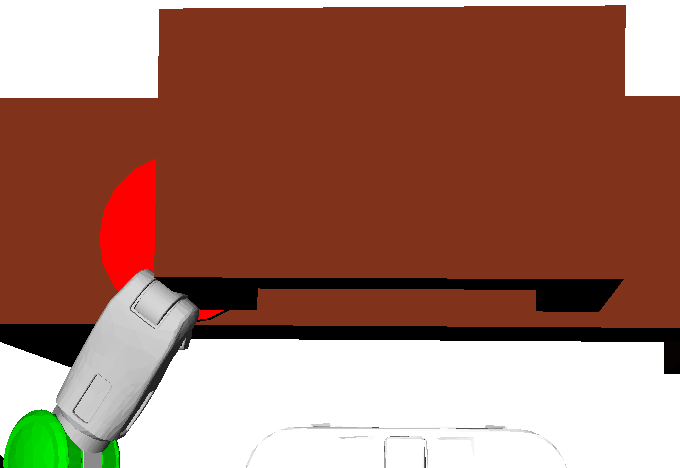
\includegraphics[scale=0.15]{images/fry_bad_grasp_pd1.png}\hspace{6mm}
%     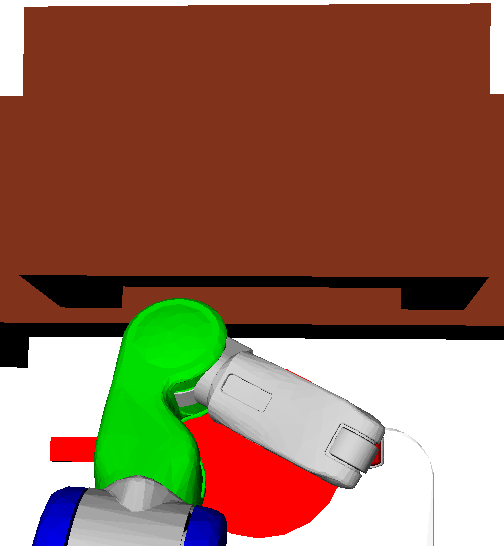
\includegraphics[scale=0.15]{images/fry_bad_grasp_pd2.png}
%     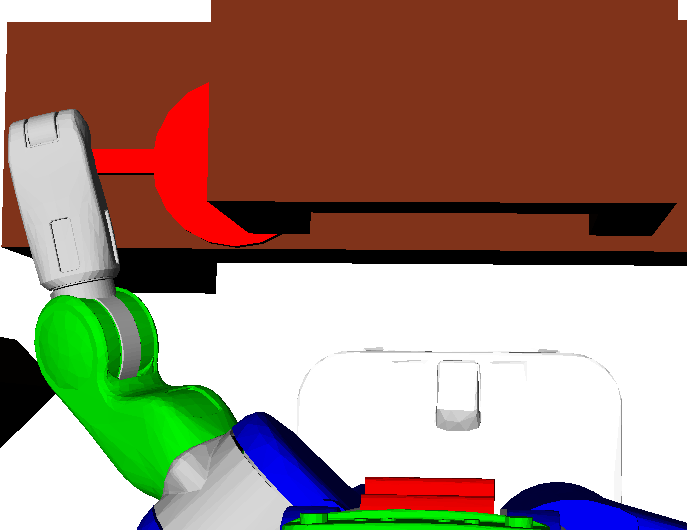
\includegraphics[scale=0.16]{images/fry_good_grasp_bad_pd.png}\hspace{6mm}
%     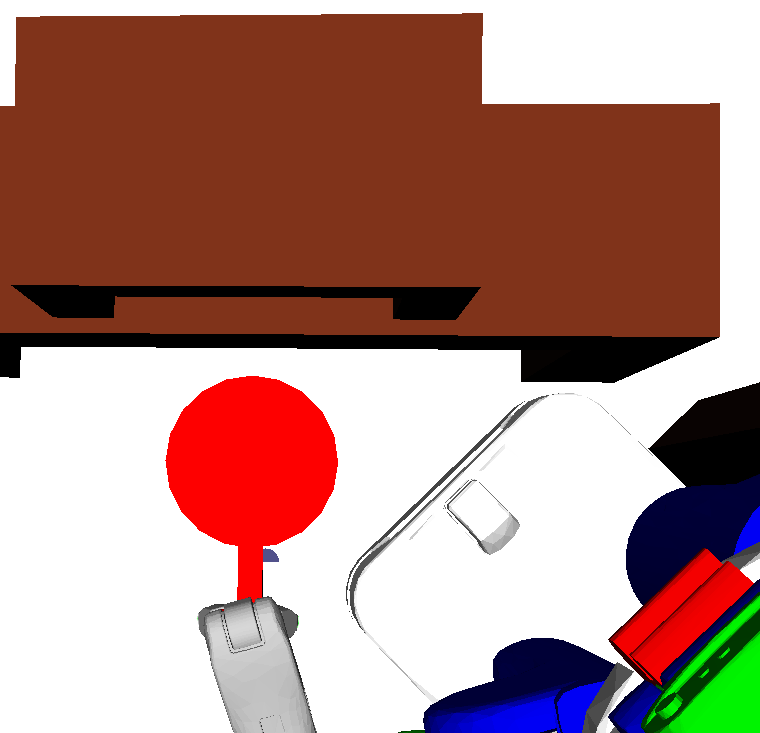
\includegraphics[scale=0.13]{images/fry_good_grasp_good_pd.png}
%   \caption{\small{\textbf{Top}: When the frying pan is not grasped by the handle, any attempted putdown pose for
% placing it into the narrow shelf fails. \textbf{Bottom}: When the frying pan is grasped by the handle, some putdown
% poses may succeed, as in the right, and some may fail, as in the left. In general, delayed rewards
% are important in the plan refinement {\sc mdp}; sometimes multiple symbolic references require resampling to
% change an infeasible refinement into a feasible one.}}
%   \label{fig:delayed}
% \end{figure}

\subsection{Training Process}
We restrict our attention to training policies that suggest $x$ for a
given parameter, since our refinement algorithm defines a way to select
$p$. Our approach is to adapt the method of Zucker et
al.~\cite{workspacebias}, which uses a linear combination of features
to define a distribution over poses. We learn a weight vector
$\theta_{p}$ for each reference \emph{type}, comprised of a pose type
and possibly a gripper (e.g., ``left gripper grasping pose,'' ``right
gripper putdown pose,'' ``base pose'').

We use a feature function $f(s, a) = f(s, p, x)$ that maps the current
state $s \in \St$ and action $a \in \A$ to a feature vector; $f$
defines a policy class for the {\sc mdp}. Additionally, we define $N$
as the number of planning problems on which to train and $\epsilon$ as
the number of samples comprising a training episode, after which we
update weights.

The training is a natural extension of randomized refinement and
progresses as follows. $N$ times, sample from $\Prob$ to obtain a
complete planning problem $\Pi$. For each $\Pi$, compute a high-level plan
and run randomized refinement to attempt to find a valid
plan refinement. Select actions according to the $\theta_{p}$ and
collect rewards according to $R$. After every $\epsilon$ calls to
\textsc{Resample}, take a gradient step on $\theta_{p}$.

For a symbolic reference $p$, in state $s$, our policy selects a
sample value $x$ with probability
$$q(s, p, x) \propto \exp(\theta_{p}^{\top} f(s, p, x)).$$

We define the expected reward of an episode, $\xi$, as
$\eta(\theta_{p})~=~\mathbb{E}_{q}[R(\xi)],$ and approximate its
gradient:
$$\nabla \eta(\theta_{p}) \approx \frac{R(\xi)}{\epsilon}
\sum_{i=1}^{\epsilon}(f(s, p, x_{i}) - \mathbb{E}_{q,s}[f]).$$
$R(\xi)$ is the sum over all rewards obtained throughout $\xi$, and
$\mathbb{E}_{q,s}[f]$ is the expected feature vector under $q$ in
state $s$. Then, for an appropriate step size $\alpha$ the weight
vector update is:
$$\theta_{p} \leftarrow \theta_{p} + \alpha \nabla \eta(\theta_{p}).$$

We sample $x$ from $q$ using the Metropolis algorithm~\cite{chib1995understanding}.
Since our distributions are continuous, calculating $\mathbb{E}_{q,s}[f]$ is hard,
so we approximate it with a Monte Carlo estimate.

\section{Experiments}
\begin{table}[t]
  \centering
  \vspace{8pt}
  \tabcolsep=0.11cm{
  \begin{tabular}{ccccc}
    \toprule[1.5pt]
      \textbf{\# Objects} & \textbf{System} & \textbf{\% Solved (SD)} & \textbf{Avg Ref Time (s)} & \textbf{Avg \# MP Calls}\\
    \midrule[2pt]
      30 (can) & T & 42 (0) & 6.2 & 8.0\\
    \midrule
      30 (can) & B & 40 (0) & 20.5 & 10.5\\
    \midrule
      30 (can) & L & 72 (8.2) & 20.4 & 11.3\\
    \midrule
      30 (can) & F & 81 (3.0) & 17.9 & 12.7\\
    \midrule[1.5pt]
      35 (can) & T & 50 (0) & 9.2 & 8.0\\
    \midrule
      35 (can) & B & 50 (0) & 17.6 & 9.2\\
    \midrule
      35 (can) & L & 68 (8.3) & 11.6 & 6.6\\
    \midrule
      35 (can) & F & 78 (2.2) & 10.6 & 6.8\\
    \midrule[1.5pt]
      40 (can) & T & 34 (0) & 19.7 & 10.3\\
    \midrule
      40 (can) & B & 36 (0) & 21.7 & 10.0\\
    \midrule
      40 (can) & L & 61 (6.3) & 18.7 & 9.4\\
    \midrule
      40 (can) & F & 74 (3.2) & 20.7 & 10.4\\
    \midrule[2pt]
      2 (dinner) & T & 100 (0) & 35.5 & 60.2\\
    \midrule
      2 (dinner) & B & 100 (0) & 37.3 & 59.2\\
    \midrule
      2 (dinner) & L & 99 (1.8) & 41.5 & 61.6\\
    \midrule[1.5pt]
      4 (dinner) & T & 100 (0) & 43.2 & 98.0\\
    \midrule
      4 (dinner) & B & 90 (0) & 63.0 & 95.5\\
    \midrule
      4 (dinner) & L & 99 (0.6) & 69.2 & 97.1\\
    \midrule[2pt]
      2 (frying) & T & 96 (0) & 29.0 & 67.2\\
    \midrule
      2 (frying) & B & 88 (0) & 46.9 & 60.0\\
    \midrule
      2 (frying) & L & 99 (2.0) & 22.6 & 44.7\\
    \midrule[1.5pt]
      4 (frying) & T & 55 (0) & 48.9 & 131.8\\
    \midrule
      4 (frying) & B & 20 (0) & 187.9 & 155.5\\
    \midrule
      4 (frying) & L & 92 (6.8) & 90.6 & 120.9\\
    \bottomrule[1.5pt]
  \end{tabular}}
  \caption{\small{Percent solved and standard deviation, along with time spent refining and number of calls to the motion
planner for baseline 1 (T), baseline 2 (B), our learned refinement policies with the graph search used in baseline 2 (L),
and our full system: learned refinement policies and graph search heuristics (F). Results for L and F
are averaged across 5 separately trained sets of weights. As described, we only run F for the can domain. Time limit: 300s.}}
  \label{table:results}
  \vspace{-1em}
\end{table}

\subsection{Methodology}
We evaluate our approach in three distinct domains: cans distributed randomly on a table (the \emph{can domain}),
setting up bowls for dinner (the \emph{dinner domain}), and placing frying pans into a narrow shelf (the \emph{frying domain}).
We compare performance with two baselines, both of which use the hand-coded refinement distributions used in {\sc sfrcra-14}.

Baseline 1 is {\sc sfrcra-14}: it uses exhaustive backtracking search for refinement
and greedy depth-first search of the {\sc prg}, which always tries to refine
the plan that incorporates all error information obtained thus far.
Baseline 2 uses randomized refinement with the following fixed graph search policy: try 3 times to refine the deepest
node in the graph; if unsuccessful, generate a geometric error, replan with the task planner (which creates a child node), and repeat.

For the can domain, we report results for 4 systems: 1) baseline 1; 2) baseline 2; 3) our learned refinement policies
with the graph search used in baseline 2; and 4) our full system, with learned refinement policies and graph search heuristics.
For the dinner domain and frying domain, we report results only for the first 3 systems, because the errors propagated in these
domains relate to the stackability of objects. Since this is independent of the current refinement, we want to
incorporate all available error information when attempting refinement. Thus, the graph search strategy
from baseline 2 can be expected to perform well in these settings.

For refinement distributions, initial experimentation revealed that training weights for all reference types jointly is intractable,
because planning takes a long time. So, we apply curriculum learning by training with a planning problem distribution
$\Prob$ that gets progressively harder. The details of this curriculum are described in each experiment's section.
Additionally, we train the refinement policies first, then fix them while collecting demonstrations and training the graph search heuristics.
For the fourth system, we reduce variance in the learning as follows. We train 3 sets of refinement weights independently,
test each one on a validation set, and output the best-performing one. We set $\alpha = 0.1$.

We report results on fixed test sets of 50 randomly generated environments for the can and dinner domains,
and 20 for the frying domain (because these environments have less variation).
For the third and fourth systems, we average results across running the training
process 5 times independently and evaluating each final set of weights.

For training refinement distributions, our weight vectors $\theta_{p}$ are initialized to $\vec{\mathbf{0}}$ for each symbolic reference type.
We use 24 features. 9 binary features encode the bucketed distance between the sample
and target object. 9 binary features encode the bucketed sample height. 3 features
describe the number of other objects within discs of radius 7, 10, and 15 centimeters around the
sample. 3 binary features describe the angle made between the vector from the
robot to the target and the vector from the sample to the target: whether the angle is less than
$\pi/3$, $\pi/2$, and $3\pi/4$.

For training graph search, we use the following feature vector $f(n)$ for a {\sc prg} node storing a high-level plan.
We first consider features of a single grasp action, targeted
at an object $o$. Consider a cone ranging from angles $-\frac{\pi}{3}$ to $\frac{\pi}{3}$
toward the closest table edge from $o$. The first feature, exists\_obstr, is a binary variable indicating
whether any other objects lie in this cone. The second, exists\_path, is a binary variable indicating whether there is a linear
grasp path wide enough for the robot's gripper to fit through within the cone. For the third feature, we approximate the robot's arm and gripper with a cylinder $c$ and sweep it across 10 discretized angles from $-\frac{\pi}{3}$ to
$\frac{\pi}{3}$. We then store the minimum number of collisions with $c$ as the feature, sweep\_count. This gives us a coarse approximation for the minimum number of objects that should be moved before the target object is accessible via a linear path.
We construct these features for the first five grasp actions in the plan, padding with -1.
We then add on the following aggregate features associated with the entire plan: 1) the minimum exists\_obstr across all grasp actions,
2) the sum of sweep\_count across all grasp actions, 3) the number of times $n$ was picked for refinement,
and 4) the number of times $n$ was picked for generating an error.

Our experiments are conducted in Python 2.7 using the OpenRave simulator~\cite{Diankov_2008_6117} with a PR2 robot.
The motion planner we use is trajopt~\cite{schulman2013finding}, and the task planner is Fast-Forward~\cite{FF}.
The experiments were carried out in series on an Intel Core i7-4770K machine with 16GB RAM.
Table \ref{table:results} summarizes our quantitative results.

% \begin{figure}[t]
%   \centering
%   \begin{subfigure}[b]{0.35\linewidth}
%     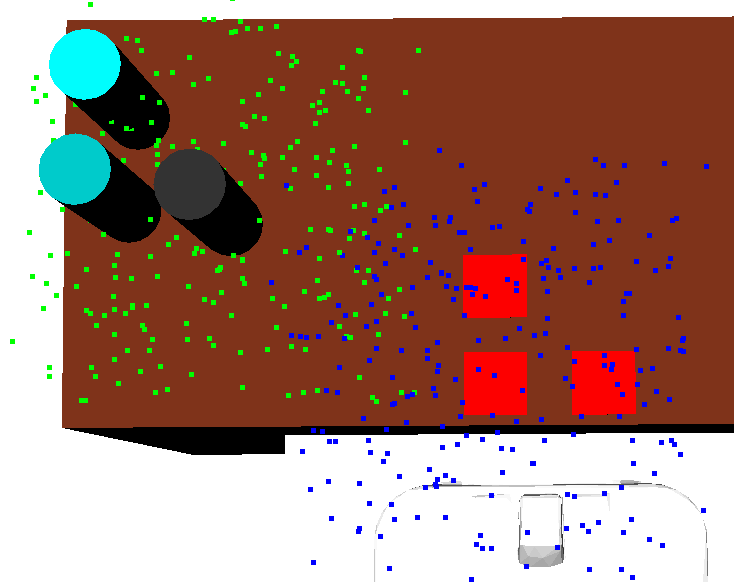
\includegraphics[width=\textwidth]{images/learns.png}
%     \caption{Initial distributions.}
%   \end{subfigure}
%   \begin{subfigure}[b]{0.35\linewidth}
%     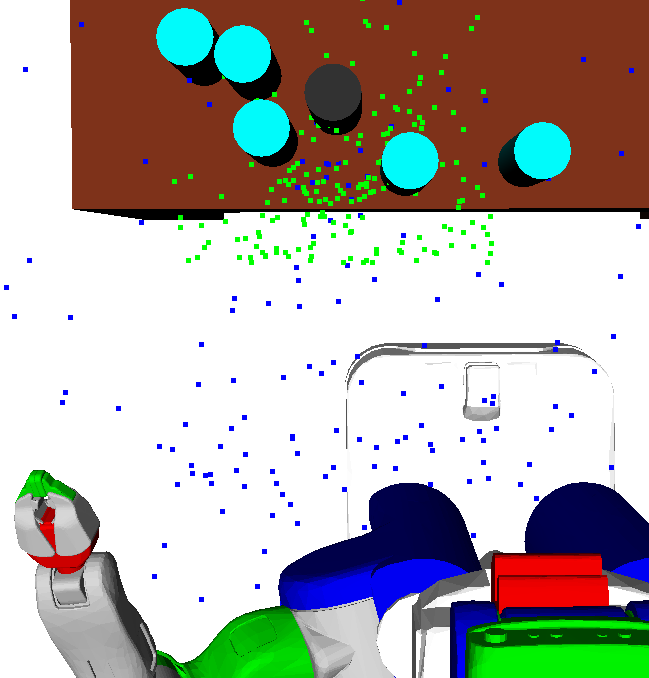
\includegraphics[width=\textwidth]{images/learn4.png}
%     \caption{After 4 iterations.}
%   \end{subfigure}
%   \begin{subfigure}[b]{0.35\linewidth}
%     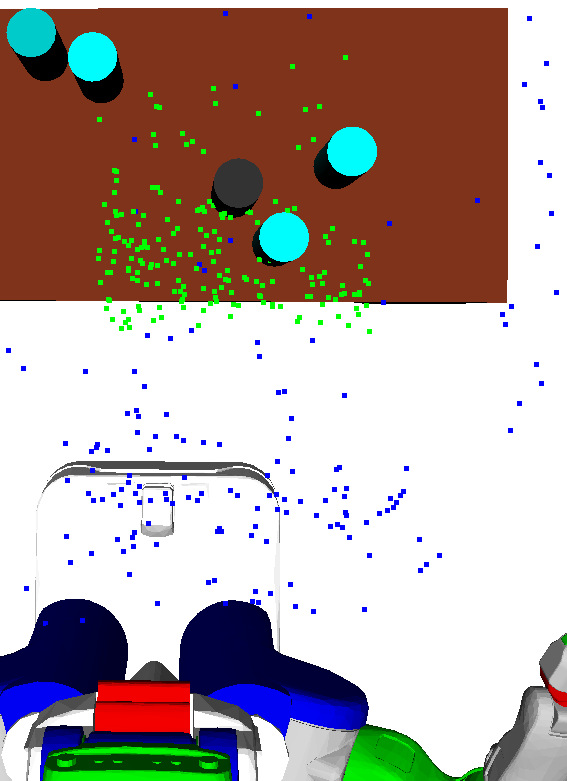
\includegraphics[width=\textwidth]{images/learn8.png}
%     \caption{After 8 iterations.}
%   \end{subfigure}
%   \begin{subfigure}[b]{0.35\linewidth}
%     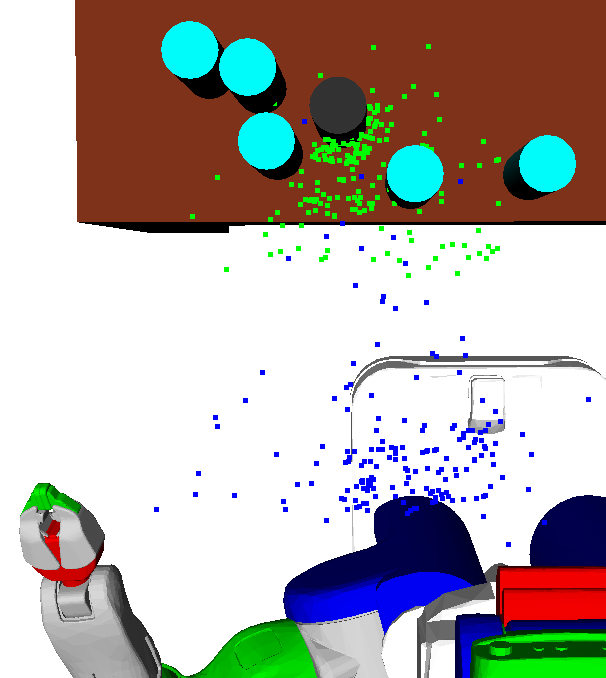
\includegraphics[width=\textwidth]{images/learn12.png}
%     \caption{Final distributions.}
%   \end{subfigure}
%   \caption{\small{Learned base position (blue) and left arm grasp (green) distributions used to
% pick up the black can after different training iterations for learning refinement policies.
% An iteration refers to a single planning problem,
% which terminates after $H$ calls to the \textsc{Resample} routine.
% Initial distributions are uniform because we initialize weights to $\vec{\mathbf{0}}$.
% Final distributions are after 12 iterations.}}
%   \label{fig:training}
% \end{figure}

\subsection{Can Domain}
We run three sets of experiments, using 30, 35, and 40 cans on the table.
The goal is always for the robot to pick up a particular can with its
left gripper. We disable the right gripper, so any obstructions to the target object must be picked up and
placed elsewhere on the table. This domain has 4 types of continuous references: base poses, object grasping
poses, object putdown poses, and object putdown locations.
% The range of allowable values for grasping and putdown poses is a cube of side length 30 centimeters around the
% target object or putdown location. For base poses, the range is a square of side length 1 meter around the
% object or location which the robot is approaching. For putdown locations, the range is defined by the table.

Our curriculum learning system first trains base poses and grasping poses for $N = 12$ iterations with $\epsilon = 5$,
then base poses, grasping poses, and putdown poses (at fixed location) for $N = 18$ iterations with $\epsilon = 20$,
then all reference types for $N = 30$ iterations with $\epsilon = 20$. We fix $H = 100$.

To train the graph search heuristics,
we collect approximately 300 optimal actions from the human demonstrator, over 3 rounds of {\sc DAgger}. After these 3 rounds,
we found that performance plateaued. We use $C = 10^{9}$ in solving the maximum-margin optimization problem.

\begin{figure}[t]
  \centering
    \noindent
    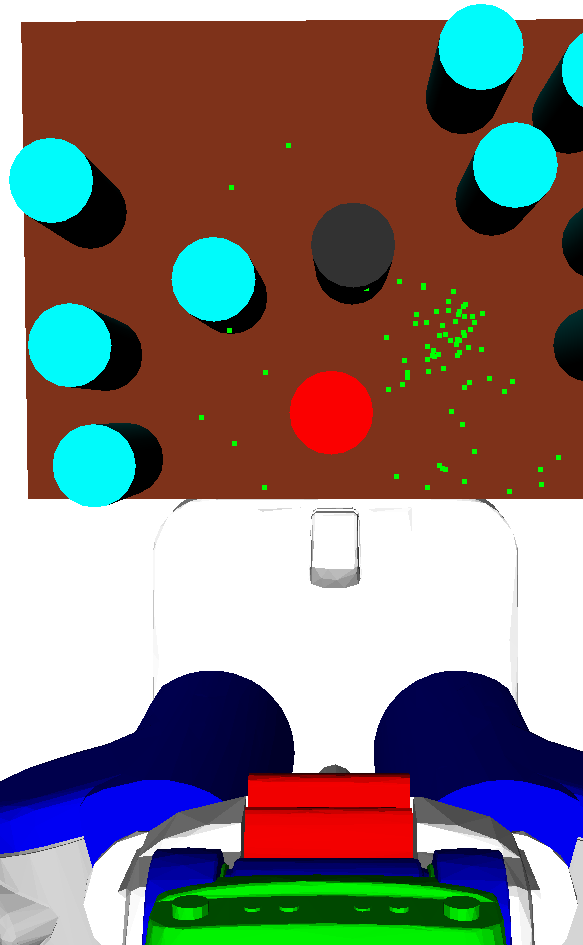
\includegraphics[scale=0.2]{images/grasp_context_1.png}
    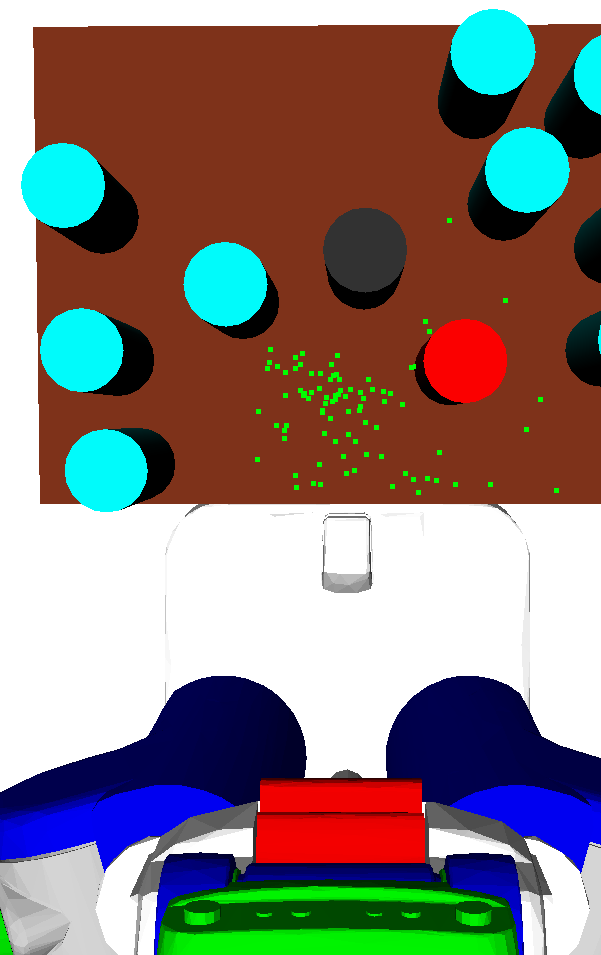
\includegraphics[scale=0.2]{images/grasp_context_2.png}
    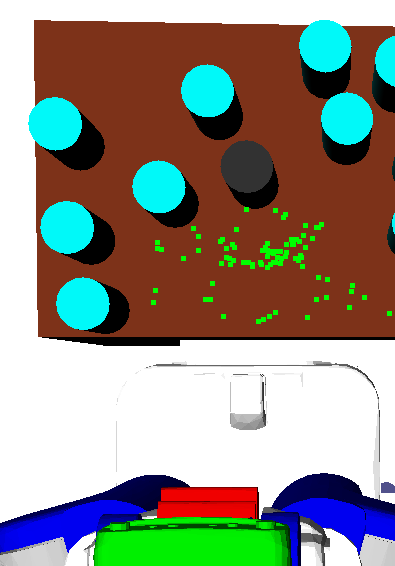
\includegraphics[scale=0.2]{images/grasp_context_3.png}
  \caption{\small{The learned left arm grasping (green) distribution for the black can is affected significantly
by the position of obstructing objects. The points refer to the position of the left tool center point; the gripper
is oriented toward the black can.}}
  \label{fig:context}
\end{figure}

The results demonstrate significant improvements in performance to the baseline systems for success rate.
However, backtracking search provides faster average refinement time. This is likely because
refinement times were averaged over the test cases where all 4 systems succeeded. These plans tended
to be easier to refine, so exhaustive backtracking search performs well because the total search space is small.
\figref{fig:cover} shows learned base motion and pickup distributions. \figref{fig:context} shows
that our system learned to shape distributions based on the geometry of the environment in which an action
is performed. The grasping distribution learned to shift away from obstructing objects, increasing robustness.

% \begin{figure}[t]
%   \centering
%   \begin{subfigure}[b]{0.45\linewidth}
%     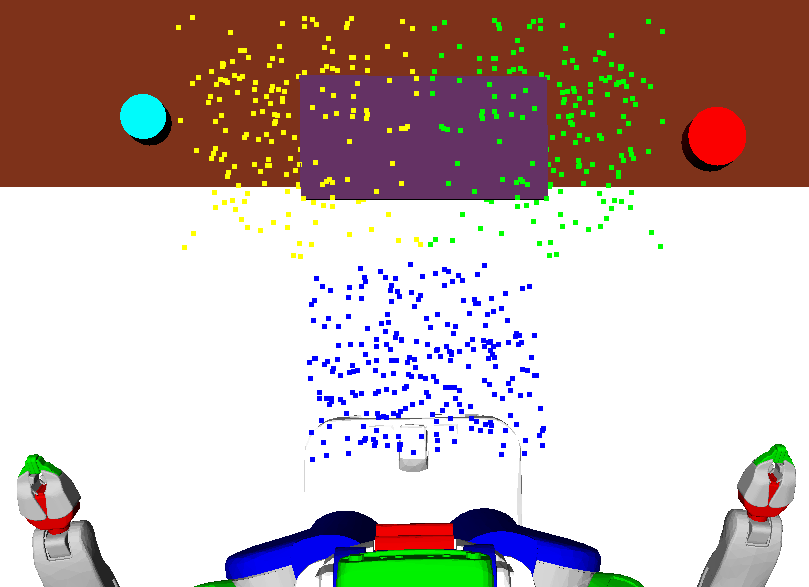
\includegraphics[width=\textwidth]{images/dinner_tray_initial.png}
%     \caption{Initial distributions.}
%   \end{subfigure}
%   \begin{subfigure}[b]{0.45\linewidth}
%     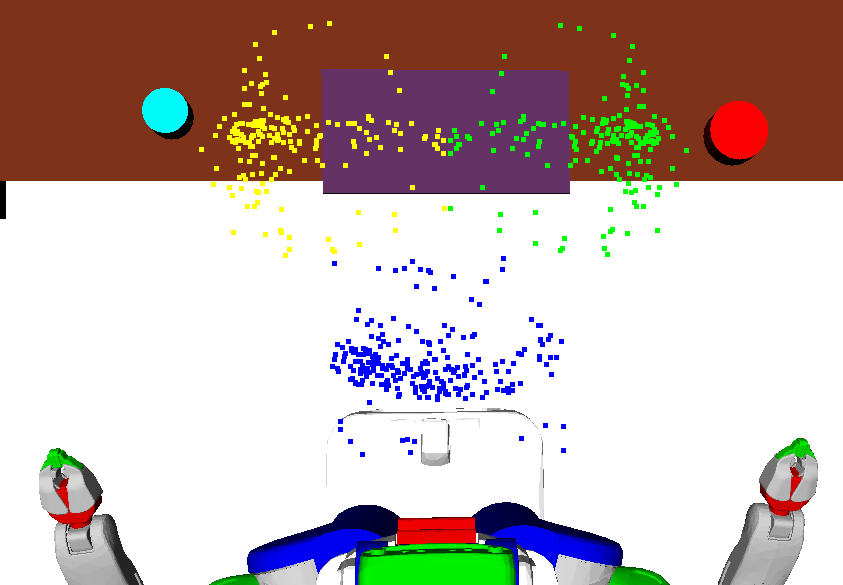
\includegraphics[width=\textwidth]{images/dinner_tray_final.png}
%     \caption{Final distributions.}
%   \end{subfigure}
%   \caption{\small{Initial and learned base position (blue) and tray pickup (green, yellow) distributions
% for the dinner domain. The green points refer to the position of the right tool center point; the gripper
% is oriented toward the tray. The left gripper is placed in a symmetric position on the other side of
% the tray, as marked by the yellow points. Final distributions are after 20 iterations.}}
%   \label{fig:dinner}
% \end{figure}

\subsection{Dinner Domain}
We run two sets of experiments, using 2 and 4 bowls. The robot must move the
bowls from their initial locations on one table to target locations on the other. We assign a cost to
base motion in the environment, so the robot is encouraged to use the provided tray, onto which bowls can be stacked.
This domain has 5 types of continuous references: base poses, object grasping poses, object putdown poses, tray pickup
poses, and tray putdown poses.

Our curriculum learning system first trains base poses and tray pickup and putdown poses for
$N = 20$ iterations, then object grasping and putdown poses for $N = 20$ iterations. We fix $H = 100$ and $\epsilon = 10$.

The results demonstrate comparable performance to the baseline systems. The reason is that
hand-coding the sample space works well in this domain. For example, the optimal
robot base pose from which to pick up the tray is directly in front of it, which is quickly sampled in
the baseline systems. Additionally, the lack of long-term dependencies in the plan
means that backtracking search finds a valid refinement quickly. The fact that our system performs comparably
with the baselines shows that our learning algorithm can recover good hand-coded distributions.
\figref{fig:cover} shows learned tray pickup poses after all 20 iterations.

% \begin{figure}[t]
%   \centering
%   \begin{subfigure}[b]{0.25\linewidth}
%     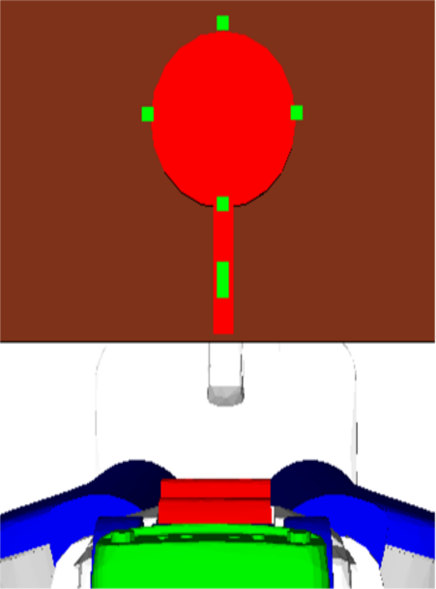
\includegraphics[width=\textwidth]{images/frying_hand.png}
%     \caption{Hand-coded distribution.}
%   \end{subfigure}
%   \begin{subfigure}[b]{0.25\linewidth}
%     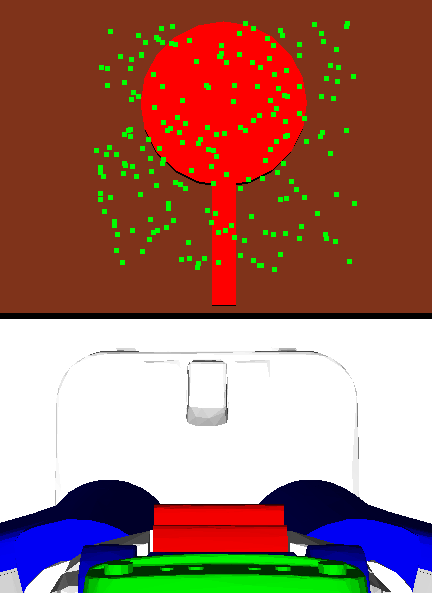
\includegraphics[width=\textwidth]{images/frying_initial.png}
%     \caption{Initial distribution.}
%   \end{subfigure}
%   \begin{subfigure}[b]{0.25\linewidth}
%     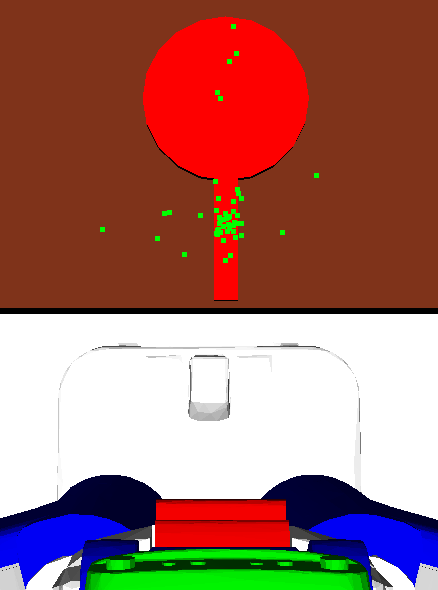
\includegraphics[width=\textwidth]{images/frying_final.png}
%     \caption{Final distribution.}
%   \end{subfigure}
%   \caption{\small{Hand-coded distribution, along with initial and final distributions using our training methods,
% for picking up the frying pan. The green points refer to the position of the tool center point; the end
% effector is oriented downward. Our system learned to prefer picking up the pan at its handle to fit it into the shelf (not shown). Final distributions are after 20 iterations.}}
%   \label{fig:frying}
% \end{figure}

\subsection{Frying Domain}
We run two sets of experiments, using 2 and 4 frying pans. The robot must stack the frying pans in order of decreasing
radius into a narrow shelf. To be successful, it must grasp the frying pans at the handle, so that the handle sticks out
after the pan is placed in the shelf. This domain has 3 types of continuous references: base poses, pan grasping poses, and
pan putdown poses. We do not use curriculum learning, as weights for all these parameters can be trained jointly.
We fix $N = 30$, $H = 100$, and $\epsilon = 5$. {\sc sfrcra-14} did not have a frying domain, so we use the following
hand-coded distribution for picking up the pans: 4 grasping poses in the cardinal directions around the lip of the pan,
and 4 equidistant along the handle.

The results demonstrate significantly higher success rate versus the baseline systems. The backtracking baseline is faster likely because
the refinement times were averaged over cases where all 3 systems succeeded; backtracking often succeeded only when
it ``got lucky'' and picked grasping poses along the handle early in the search. \figref{fig:cover} shows learned frying pan
grasping poses after all 30 iterations. Our system learned to prefer picking up the pan at its handle to fit it into the shelf, which is not shown.

\section{Conclusion and Future Work}
We presented a novel application of reinforcement learning to plan refinement in task
and motion planning. Our method trained a policy for refining symbolic plans
by learning good sampling distributions for plan parameters. The choice
of which parameter to resample at each iteration was governed by a novel
refinement strategy we presented called randomized refinement. We evaluated
performance by comparing against a baseline of hand-coded distributions
for several challenging pick-and-place tasks. Our system demonstrated overall comparable
to improved performance in motion planning time and number of motion planner calls.

One important direction for future work is improving the feature vector to incorporate
information about the symbolic plan and previous samples of a parameter.
Another is training a system that decides
whether to return to the high level on its own, instead of relying on
reaching the iteration limit in the randomized refinement algorithm. This would
make the training optimize more directly for producing a valid refinement,
given an arbitrary task planning problem.

%\addtolength{\textheight}{-12cm}   % This command serves to balance the column lengths
                                  % on the last page of the document manually. It shortens
                                  % the textheight of the last page by a suitable amount.
                                  % This command does not take effect until the next page
                                  % so it should come on the page before the last. Make
                                  % sure that you do not shorten the textheight too much.

%%%%%%%%%%%%%%%%%%%%%%%%%%%%%%%%%%%%%%%%%%%%%%%%%%%%%%%%%%%%%%%%%%%%%%%%%%%%%%%%



%%%%%%%%%%%%%%%%%%%%%%%%%%%%%%%%%%%%%%%%%%%%%%%%%%%%%%%%%%%%%%%%%%%%%%%%%%%%%%%%



%%%%%%%%%%%%%%%%%%%%%%%%%%%%%%%%%%%%%%%%%%%%%%%%%%%%%%%%%%%%%%%%%%%%%%%%%%%%%%%%
\bibliography{$LATEXROOT/references}

\end{document}
